%; whizzy chapter
% -initex iniptex -latex platex -format platex -bibtex jbibtex -fmt fmt
% 以上 whizzytex を使用する場合の設定。

%     Tokyo Debian Meeting resources
%     Copyright (C) 2007 Junichi Uekawa

%     This program is free software; you can redistribute it and/or modify
%     it under the terms of the GNU General Public License as published by
%     the Free Software Foundation; either version 2 of the License, or
%     (at your option) any later version.

%     This program is distributed in the hope that it will be useful,
%     but WITHOUT ANY WARRANTY; without even the implied warranty of
%     MERCHANTABILITY or FITNESS FOR A PARTICULAR PURPOSE.  See the
%     GNU General Public License for more details.

%     You should have received a copy of the GNU General Public License
%     along with this program; if not, write to the Free Software
%     Foundation, Inc., 51 Franklin St, Fifth Floor, Boston, MA  02110-1301 USA

%  preview (shell-command (concat "evince " (replace-regexp-in-string "tex$" "pdf"(buffer-file-name)) "&"))
% 画像ファイルを処理するためにはebbを利用してboundingboxを作成。
%(shell-command "cd image200708; ebb *.png")

%%ここからヘッダ開始。

\documentclass[mingoth,a4paper]{jsarticle}
\usepackage{monthlyreport}

% 日付を定義する、毎月変わります。
\newcommand{\debmtgyear}{2007}
\newcommand{\debmtgdate}{18}
\newcommand{\debmtgmonth}{8}
\newcommand{\debmtgnumber}{31}


\begin{document}

\begin{titlepage}

% 毎月変更する部分, 本文の末尾も修正することをわすれずに

 第\debmtgnumber{}回 東京エリア Debian 勉強会資料

\vspace{2cm}

\begin{minipage}[t]{0.6\hsize}
\vspace{-2cm}
{\fontsize{60}{60}
{\gt
\color{dancerdarkblue}
東京エリア \\
デビアン \\
勉強会
}}
\end{minipage}
\begin{minipage}[b]{0.4\hsize}
\hspace{-1cm}
\includegraphics[width=9cm]{image200502/openlogo-nd.eps}
\end{minipage}

\vspace{3cm}
\hfill{}Debian勉強会幹事 上川 純一\\
\hfill{}\debmtgyear{}年\debmtgmonth{}月\debmtgdate{}日

\thispagestyle{empty}
\end{titlepage}

\dancersection{Introduction}{上川 純一}


今月のDebian勉強会へようこそ。
 これからDebianのあやしい世界に入るという方も、すでにどっぷりとつかってい
 るという方も、月に一回Debianについて語りませんか?

 目的として次の二つを考えています。

 \begin{itemize}
 \item メールではよみとれない、もしくはよみとってられないような情報につ
       いて情報共有する場をつくる
 \item Debianを利用する際の情報をまとめて、ある程度の塊として整理するた
       めの場をつくる
 \end{itemize}

 Debianの勉強会ということで究極的には参加者全員がDebian Packageをがりがり
 と作るスーパーハッカーになった姿を妄想しています。

 Debianをこれからどうするという能動的な展開への土台としての空間を提供し、
 情報の共有をしたい、というのが目的です。


\newpage

\begin{minipage}[b]{0.2\hsize}
 \colorbox{dancerlightblue}{\rotatebox{90}{\fontsize{80}{80} 
{\gt \color{dancerdarkblue}デビアン勉強会}}}
\end{minipage}
\begin{minipage}[b]{0.8\hsize}
\hrule
\vspace{2mm}
\hrule
\setcounter{tocdepth}{1}
\tableofcontents
\vspace{2mm}
\hrule
\end{minipage}

\dancersection{事前課題}{上川 純一}

今回の事前課題は
「ここ最近 Debian を使っていて ハマったこと/ちょっと感激したこと」もしく
は「apt の sources.list はこう書く」
というタイトルで200-800文字程度の文章を書いてください。というものでした。
その課題に対して下記の内容を提出いただきました。

\subsection{小室 文}

\subsubsection{ここ最近 Debian を使っていて ハマったこと/ちょっと感激したこと}

あんまりDebian特有ではないけど、Gimpってかなり使える事が判明して、結構感
動しました。元々MacでAdobe Photoshop/Illustratorを使っていたのですが、メ
インPCもDebianになったので、Gimpを使ってみようとあれこれしているうちに
Gimpってイイ!という事が判明。かなり使えるやつです。
後普通の人は知ってて当り前かもしれないけどgnome-utilsはなんかお得感一杯
(でもないけど)なパッケージでこういうのは結構小さな感動があったりします。

\subsection{根岸 心}

\subsubsection{感動したこと}

開発環境を用意しようと、家に転がっていたPentiumIIのマシンにsargeをインストールしたのが、Debianとの出会いです。本番環境も当然Debianを使おうと思って、DELLのSC430を購入した後に、etchが登場したばかりで、安定的にSC430上で動作するDebianが無いことに気づき、仕方なくCentOSを利用することにしました。その時から、開発環境はDebian、本番環境(SC430)はCentOSで運用しています。CentOSマシンが増えてしまい、etchに全面移行することに踏み切れないため、CentOSをいじっている時間が長いですが、Debianマシンに戻る度に、あるべきところにあるべきファイルがある、通っているべきパスが通っていることに感動します。


\subsection{Tsukasa Hamano}

\subsubsection{ここ最近 Debian を使っていて ハマったこと/ちょっと感激したこと}

最近自宅にオレオレaptレポジトリを作った事でお気に入りの環境が素早く構築
できるようになってちょこっと感動しました。

あと libdwarf-dev というライブラリのパッケージが sarge まであったのに
etch から無くなっていて悔しい思いをしたのですが、今日 libdw-dev という
同等のライブラリを見つけてマジで感激しました。

\subsubsection{apt の sources.list はこう書く}

\url{sources.list} はたくさん書くと update が遅くなって我慢できなくなるので

\begin{commandline}
 % m4 -DDIST=etch /etc/apt/sources.list.m4 > /etc/apt/sources.list
\end{commandline}

などと細かく分けた apt-line をその都度生成したり、symlink で切り替えた
りしていました。もっとカッコイイ方法があるんじゃないかと確信しています。

\subsection{前田 耕平}

\subsubsection{ここ最近 Debian を使っていて ハマったこと/ちょっと感激し
   たこと}

テストではまって、家サーバをいまだにSargeからEtchに移行できていません。orz
久々に時間ができたので、Etchで構築したOpenBlocks266で、下記のように移行
しようと、Etchで環境作りました。

現状:Sarge\\
Apache 2.0 + mod\_php + PHP4 + PukiWiki + mod\_security 1.8

移行後の予定:Etch\\
Apache 2.2 + mod\_fcgid + PHP5 + PukiWiki + mod\_security 2.0

んで、phpinfo()はちゃんと結果を返すのに、PukiWikiでindex.phpにアクセスすると、failed
fopenでこけてしまうので、困ってしまったなぁと。
パッケージをそのまま使うのならaptitude update;aptitude
dist-upgradeでも良いのかもしれませんが、カスタマイズしている部分があるので、時間を割いて検証してみます。(いつだ?)
他のサーバもWebサーバが終わらないと検証できないので、Pending…。臆病者なので、いきなりアップグレードだなんてできません。w

ところで、PukiWikiってなぜパッケージないんでしょうね。別に必要はありませんけど。


他は、クライアントとしてSidを使っていてアップデートによって環境がおかしくなってしまっても、そのまま使っていたら結構馴れてしまうんだということに気がつきました。ダメ人間です。

\subsubsection{apt の sources.list はこう書く}

とくにないです。通常と違うのは、自宅のHobbit
monitorのサーバ&エージェントや、自宅鯖を運用するのに共通で使っているスクリプトを配布するのに、自宅のLANで立てているリポジトリを追加している程度です。

\subsection{ARAKI Yasuhiro}

\subsubsection{apt の sources.list はこう書く}
\begin{commandline}
 deb http://cdn.debian.or.jp.nyud.net:8090/debian/ sid main
\end{commandline}

と書くことがたまにあります。\url{cdn.debian.or.jp}を他に変えても日本では速くないので
意味がありませんね。。

日本にいるときは

\begin{commandline}
 deb http://cdn.debian.or.jp/debian/ sid main
 deb-src http://cdn.debian.or.jp/debian/ sid main
\end{commandline}

ですね。etchまではjavaがなかったので行追加していましたが、現在は
変なツールをいれてないのでこれで十分です。

\subsection{Hisashi MORITA}

\subsubsection{ここ最近 Debian を使っていて ハマったこと/ちょっと感激したこと}

久しぶりに新規インストールしたら、\url{/etc/default/locale}があるのに気が付か
ずはまりました。
また少し前ですが、teTeXからTeXLiveへ大きな問題なく移行できたのには感心し
ました。

\subsubsection{apt の sources.list はこう書く}

うまく書けないのでbest practiceを知りたいところです。

\subsection{山根秀樹}

\subsubsection{ここ最近Debian を使っていてハマったこと}
\begin{itemize}
 \item ハマったというか、シャットダウン時に必ず kernel log daemon が failed します。
 何故でしょう?
 \item 2.6.21 あたりから cpufreq なモジュールの読み込みに失敗します。なんか変更必要
 だったかな?
 \item util-linux でなんか含まれてないの (flock) があるぞ、というのをきんねこさんが書
 いていたので自前で修正してビルドしようとしたら、aclocal,automake,autoconf が入っ
 ている環境だとビルドにこけるという状態に陥った。何で誰も直してないんだこれ。
 \item bcm43xx な無線LANカードを使っているのですが、2.6.18 までは問題なかったのに、そ
 れ以降(2.6.21、2.6.22など) が極度にスピードが遅くなった(タイムアウトもざら。ど
 うやら中身をまるっと書き換えてあるかららしいんですが、ドライバ側の対応待ちなのか
 なー?)
 \item tar のオプションを見ようとしたら、日本語の man になかった→LAMG=C で元の man を
 見ると新しい…でも GFDL のために Debian で新しく作ったものだった→infoを見てみる→
 日本語 info だとまともに表示されない orz
 \item ddtp で訳された description が apt で利用できるようになったのはいいのですが、
 内容が EUC-JP で書かれているために現在の UTF-8 な状態では文字化けしてまるで読め
 なかった。
 \item onscripter で「ひぐらしのなく頃に」を遊ぼうとする→一部音声が再生されない orz
 \item anthy のアップデートで辞書ファイルの参照がおかしくて「☆」が入力できなかった
 (いや、「はて☆すた」とか書きたかっただけなんです)。
 \item あまりに普段 Debian だけで作業をしていて、家の Windows を起動しないでいたらパ
 スワードを思い出せなくなりました。
\end{itemize}

普通に使っているだけなのに日々ハマっていますね。うーむ。


\subsubsection{ちょっと感激したこと}

\begin{itemize}
 \item  E-mobile なカードを借りられたので設定をしてみたら、pppconfig で設定をさくさく
 できたこと。Windows よりある意味楽かも(PPP接続なんかも gnome のネットワーク設定
 からサクッとできるといいのかな。出来るかもしれないけど試してない)。岩松さんが
 Willcom の設定をしたときに接続設定の雛形があると良いかも、などといっていたが、こ
 れは E-mobile にもいえることかも。
\end{itemize}


\subsubsection{sources.list はこう書く}

nano ではなく vi で…じゃなくて、sources.list 自体には cdn.debian.or.jp だけ書い
ています。他のものについては、/etc/apt/sources.list.d/ 以下に用途に分けて書いて
ます。で、必要なくなったら(official に入った、配布を取りやめたなどの場合)コメ
ントアウトしたり消したりしています。

\begin{commandline}
deb http://www.debian-multimedia.org sid main
\end{commandline} 
ぐらいかなぁ、追加してるのは。

\subsection{荒木 淳}

\subsubsection{apt の sources.list はこう書く}

使用 OS は、Debian etch stable です。
最初に参考文献の紹介です。以下のページを参考にしました。

\begin{itemize}
 \item   \url{http://www.debian.org/doc/manuals/apt-howto/ch-basico.ja.html}
 \item  \url{http://debian.fam.cx/index.php?install#content_1_37}
\end{itemize}

最適なミラーを探し出すのに、apt-spy と netselect-apt を使用しました。最初に、apt-spy です。

\begin{commandline}

 $ sudo apt-spy update
 $ sudo apt-spy -d etch -s JP
\end{commandline}

これにより、以下の行が自動的に sources.list に書き込まれていました。既存の sources.list は
sources.list.bakに退避されました。

\begin{commandline}
 # sources.list generated by apt-spy v3.1
 deb http://ftp.jp.debian.org/debian/ etch main
 deb-src http://ftp.jp.debian.org/debian/ etch main
 #deb http://security.debian.org/ stable/updates main
\end{commandline}

 次に netselect-apt です。

\begin{commandline}
  $ sudo netselect-apt
\end{commandline}

これにより、以下の行が自動的に sources.list に書き込まれていました。既存の sources.list は
sources.list.orig に退避されました。

\begin{commandline}
 # the main Debian packages.
 deb http://ftp.dti.ad.jp/pub/Linux/debian/ stable main contrib
 # Uncomment the deb-src line if you want 'apt-get source'
 # to work with most packages.
 # deb-src http://ftp.dti.ad.jp/pub/Linux/debian/ stable main contrib
 # uncommenting the following line will enable security updates
 #deb http://security.debian.org/ stable/updates main contrib
\end{commandline}

上記に加えて、以下の行も推奨ということで追加しておきました。

\begin{commandline}
  deb http://cdn.debian.or.jp/debian etch main contrib non-free
 deb http://ftp.debian.or.jp/debian-security etch/updates main contrib
 non-free
 deb http://security.debian.org/ etch/updates main contrib non-free
\end{commandline}

\subsection{Noriaki Sato}

\subsubsection{感動したこと}
初めて apt-get を使った時、すごく感動した(全然最近じゃない
けど、それ以外に debian で特別感動した事って無いような、、、

\subsubsection{ハマったこと}
sarge → etch の upgrade で kacpid が暴走してハマった
のは5月に話したし、

samba を install した時、
Windows からマシンのアイコンは見えているのに、
「ネットワークパスが見つかりません」と出て繋げなくてハマった
のは CentOS の話だし、、、

そう言えば、この時、
CentOS のパッケージには cfdisk と w3m が見当たらなくて、
「やっぱり debian ってパッケージ多いんだなあ」
と改めて思いました(ちょっと感動)。

あと「ハマった」のとはちょっと違うけれど、
数ヶ月前、tDiary に脆弱性が見つかった時、
package がなかなか update されなかったので、
結局、package は uninstall して
自分で手動で入れ直したとゆー事がありました。

\subsubsection{おまけ}

debian はまった OR ハマった OR はまって OR ハマって に一致する日本語のペー
ジ 約 57,200 件中 1 - 50 件目 (0.19 秒) 

debian 感動 の検索結果 約 311,000 件中 1 - 50 件目 (0.20 秒) 

debian でハマった人に対して、感動した人は 5 倍程度いるようです。
めでたしめでたし。

#先月と同じネタですいません。

\subsection{岩崎 修}

\subsubsection{ここ最近 Debian を使っていて ハマったこと/ちょっと感激したこと}
DELLのPowerEdge SC440にネットワークインストールのCDからインストールした
ところ、すっきりさっぱり、どこにもハマらずにインストール出来てしまったこ
とにちょっと感激しました。
後の様々な設定(webサーバやpostfix、などなど)もaptitudeのおかげで楽々イン
ストール。当たり前の用にwoodyの頃から使ってましたが、これは感激していい
ことなんだろうな、と思います。

\subsubsection{apt の sources.list はこう書く}
デフォルトのまま使っています。逆に、どのように書くのがスマートなのか、勉
強させていただきたいと思います。

\subsection{山下 尊也}

第5回 関西 Debian 勉強会の時に、講師の方から頂いた資料に対して、
勉強会の表紙を作ろうと思い作ったのだが、pdfで配布資料と結合する
際にpdftkがインストールを試みると、libgcjの関係でインストール
出来なかった。時間がなかったので、依存関係の解決だけだったので、
snapshot.debian.netからパッケージを持ってきてインストールを
行ったが、やはり、このようなサービスが有志によって提供されている
って素晴らしいですね。

\subsection{奥野 由紀}

\subsubsection{ここ最近 Debian を使っていて ハマったこと/ちょっと感激したこと}

実は今までDebianはちょっと敷居が高いな、と思っていました。
ですが、先日オープンソースカンファレンス.dbで
HPのサーバーが当たってしまったので、
思い切ってamd64版のetchを入れました。
(目録はGeekoのぬいぐるみだったのに……)
噂には聞いていましたが、Debian のパッケージは豊富ですね。
お題どおり「ちょっと感激」しました。
気がつけばsid + experimental にしてデスクトップPCとして常用しつつあります。
(サーバー用PCなのに……)

\subsection{キタハラ}

\subsubsection{ここ最近 Debian を使っていて、ハマったこと/
   ちょっと感激したこと}

  これまで sarge でがんばっていたのですが、今回
のお題をみて、「これは etch を入れにゃーあかんな」
ということで入れてみました。

  sarge の時は、日本語入力の設定やサウンド出力で
苦労しましたが、etch ではあっさり使用できるように
なって、YouTube も クリック一発で Flash のプラグ
インが組み込まれ、あっさり動画が再生されました!
(おぉ、感動!)

  噂の GUI インストーラも試してみましたが、なか
なかよさげで、人に勧める時に良い感じ。(個人的には
動作がキビキビしている CUI で十分だが)

\subsection{内山}

\subsubsection{ここ最近Debian を使っていてハマったこと/ちょっと感激したこと}

\begin{itemize}
 \item 玄箱でsarge $\rightarrow$ etch化があっけなく終わった事
 \item クロスdebootstrapで簡単にRFSが作成できてしまった事
\end{itemize}

\subsection{小林}

\subsubsection{ここ最近 Debian を使っていて ハマったこと/ちょっと感激したこと}

aptによる依存関係の自動解決・ソフトウェアのコマンド一発インストール・ソースコードのコマンド一発取得が当たり前になりすぎて、
Debianを使っていても感激しないのですが、
他のOSを使っているとしょっちゅうDebianのすごさに感激します。
他のOSにはもう戻れません。

\subsubsection{apt の sources.list はこう書く}
昔は色々unofficialなパッケージのためのエントリを加えていましたが、
最近ではofficialなものだけで事足りるので (素晴らしい!!) 特に改変していません。
以前はtestingにはunstable経由でしかセキュリティサポートが入りませんでしたが、
最近では\texttt{security.debian.org}の\texttt{lenny/updates}経由でも入るようになったので、
それは取り込めるようにしています。

\subsection{鈴木}

\subsubsection{ここ最近 Debian を使っていて ハマったこと/ちょっと感激し
   たこと}

Debianだからいいかな。

ハマる前の段階ですが、Debian GNU/Hurdのインストールができてません。
最初のインストールは出来て再起動後の設定がよく分からず、
ドキュメント読んでも進まず。MAKEDEVで何作ればいいの? fstabは?
使わないかも知れないけど、とりあえずインストールしてみたい。
いつの間にか楽なインストールや設定に慣れてしまった私。
勉強会までできるかどうか...

\subsubsection{apt の sources.list はこう書く}

普通のsources.listです。

\begin{commandline}
 deb http://ftp.riken.go.jp/pub/Linux/debian/debian/ unstable main
 contrib non-free
 deb-src http://ftp.riken.go.jp/pub/Linux/debian/debian/ unstable main
 contrib non-free
 deb http://www.debian-multimedia.org sid main
 deb-src http://www.debian-multimedia.org sid main
 deb http://ftp.debian-unofficial.org/debian sid main contrib non-free
 restricted
 deb-src http://ftp.debian-unofficial.org/debian sid main contrib
 non-free restricted
 ##deb http://www.mithril-linux.org/~henrich/debian/package/ ./
\end{commandline}

\subsection{David Smith}


\subsubsection{ここ最近 Debian を使っていて ハマったこと/ちょっと感激したこと}
仕事で設定ファイルをパッケージにまとめたかったなと思ってやってみたら
cdbsで意外に簡単で感動しました。以前cdbs等のツールについてお話しが
あったと思いますが誰でもできることはあまり示されなかったかもしれないので、
こんなような作ったと紹介したいです。

\subsubsubsection{"/"ファイルシステムのようなディレクトリ階層を作成。}
設定ファイルをそこで管理する。例えば~/project/shorewall-basic-settingsだったら
そこにetc/shorewallディレクトリを作って設定ファイルを格納。
僕のプロジェクトは以下の感じ、

\begin{commandline}

 $ find ~/project/shorewall-basic-settings
 .
 ./etc
 ./etc/shorewall
 ./etc/shorewall/interfaces
 ./etc/shorewall/policy
 ./etc/shorewall/rules
 ./etc/shorewall/zones
 ./etc/default/shorewall
\end{commandline}

\subsubsubsection{そのディレクトリにdebianディレクトリを作成、以下のファイルを記入}
\begin{commandline}
==./debian/rules==
#!/usr/bin/make -f
DH_ALWAYS_EXCLUDE".svn"
include /usr/share/cdbs/1/rules/debhelper.mk

==./debian/install==
etc/shorewall/*
etc/default/shorewall

==./debian/changelog==
dds-shorewall-basic-settings (1.0) unstable; urgency=low

 * Initial release of shorewall settings package.

-- David Smith <davidsmith@acm.org>  Thu, 16 Aug 2007 14:12:45 +0900

==./debian/control==
Source: dds-shorewall-basic-settings
Section: misc
Priority: extra
Build-Depends: debhelper (>= 5), cdbs
Maintainer: David Smith <davidsmith@acm.org>
Standards-Version: 3.7.2

Package: dds-shorewall-basic-settings
Architecture: all
Depends: shorewall, ${misc:Depends}
Description: Customized basic shorewall configuration for my servers
These settings set up shorewall to run allowing basic services that all
hosts should support. It blocks everything except ping, ssh, and UDP
traceroute from the outside world.

==./debian/copyright==
Copyright 2007 David Smith <davidsmith@acm.org>. Public Domain.
\end{commandline}

\subsubsubsection{終わりに}

debianディレクトリはchangelog以外ほとんど変更しないので管理しやすくて
明瞭だと思います。

\subsubsection{apt の sources.list はこう書く}
最近sources.listを空っぽにしてsources.list.dにstable.list、testing.list、
security.listなどで分別してみました。目的としてはcron-aptでsecurity.list
だけに指したり自作パッケージで専用レポジトリを追加削除したりしたかったの
ですが、結局libaptのバグらしくてsources.list.dを使っているならDir::Etc::SourcesList
を設定しても効かないみたいだったから止めてしまって新規インストールのような
綺麗にまとまったsources.listを書くことにしちゃいました。


\subsection{碇}

Debianはもっぱらサーバーとして利用しています。
メールサーバー兼webサーバーが一台、開発ようのサーバーを2台動作させていま
す。現在PHPによるサービスを開発していまして、その際の設定で躓いたことを
報告します。
開発自体はWindowsで行っていまして、IDEとしてPDTというZendが提供している
eclipseプラグインを使用しています。サーバーへのデプロイとブレークポイン
トを設定してのデバッグができるのですが、軽くはまっときました。
デプロイ自体はsamba経由で設定できたのですが、デバッグがなかなかうまくで
きませんでした。
ZendDebuggerをphp.iniに設定するさいにWindowsとLinuxで書式が違うことに
気がつかずはまりました。

\begin{itemize}
 \item Windows:
\begin{commandline}
zend_extension_ts="c:\php\ZendDebugger.so"
\end{commandline} 
\item Linux:
\begin{commandline}
zend_extension="/usr/local/lib/ZendDebugger.so"
\end{commandline}
\end{itemize}

上記のように設定しなければいけない所をDebianでWindowsの設定をしていたた
め動作しなかったのでした。




%%% trivia quiz
\dancersection{Debian Trivia Quiz}{上川 純一}

ところで、みなさん Debian 関連の話題においついていますか?Debian関連の話
題はメーリングリストをよんでいると追跡できます。ただよんでいるだけではは
りあいがないので、理解度のテストをします。

今回の出題範囲は\url{http://www.debian.org/vote/2007/vote_003} にある投票
結果と、\url{http://lists.debian.org/debian-devel-announce/} にある最近の
アナウンス文書です。

\subsection{問題}

\santaku{Debian Maintainers の提案は何をするものか}
{気に入らない Debian Developer を投票により追放する}
{Debian Developer より制限された権限をもつ Debian Maintainers を定義する}
{Debian Developer の品質を改善する}
{B}

\santaku{
Bits from the DPL: FTP assistants, DM, APT, sharing patches
で Sam Hocever が主張したのは
}
{パッチを共有しよう}
{もう会長としての仕事は終わった}
{Debian としては Ubuntu の殲滅が目標}
{A}

\santaku{
apt-get install の仕組みで大きな変化が発生したのは何か
}
{Suggests  をデフォルトでインストールするようになった}
{Recommends をデフォルトでインストールするようになった}
{Depends を無視するようになった}
{B}

\santaku{lenny のリリースゴールに入っているのはどれか}
{Debian の市場シェア40\% 以上の獲得}
{debian/rules が国際化対応}
{debian/changelog と debian/control は UTF-8}
{C}

\santaku{sparc32 になにがおきたか}
{次のリリースではサポートされなくなる}
{急にユーザが増えたので開発者を募集している}
{arm とバイナリ互換になった}
{B}

\dancersection{最近のDebian関連のミーティング報告}{上川 純一}


\subsection{東京エリアDebian勉強会30回目報告}
% (query-replace-regexp "<.*?>" "")
% (query-replace-regexp "^[ 	]*" "")

東京エリアDebian勉強会参加報告。7月の第30回東京エリアDebian勉強会を実施し
ました。

今回の参加者はIan Lewisさん、山本浩之さん、山根さん、小室文さん、前田耕平
さん、倉沢望さん、岩崎修さん、岩松信洋さん、noriaki satoさん、uchiyama
toru さん、北原さん、小林(王子)さん、hisashi morita さん、Charles
Plessy さん、吉田@板橋さん、むかい?さん、野首さん(宴会だけ参加)、上川
の 18 人でした。

まず、DWNクイズを今回も実施しました。全員に起立してもらい、グー・チョキ・
パーで選択してもらいました。みんな予習しているようで今回の正解率は非常に
高く、熱戦が繰り広げられました。最後までのこった4人に豪華景品が渡されま
した。

次に先月開催されたDebconf7 について岩松さんが報告しました。これでもう参加
者のみなさまの来年のアルゼンチン開催の Debconf8に参加する準備は万端ですね。

組込みのリアルタイムについてはどうなっているのかという質問が出ました。リ
アルタイム性能についてはDebianとしては、debian-multimediaプロジェクトが中
心に推進をすすめているのですが、組込み用途でその点を重視しているものがあ
るかどうかについては不明です。Linux Kernel の標準でリアルタイム優先度のサ
ポートなどが組み込まれているのでいけるんじゃないか?という話題がでました。
状況については確認必要ですね。オーディオに関しては有用なリアルタイム性能
が、ロボット制御の場面で有用か、一概にはいえなさそうですね、という話が展
開しました。sched\_setschedulerでSCHED\_FIFOかSCHED\_RRを設定するとリアル
タイム優先度でプロセスが実行されるはずです。

最後に上川がDebconfを日本で開催するためにはどういうことをしたらよいのか、というトピックに関して、
参加者の事前課題を紹介しながら議論しました。
Debconf7の会期は一週間以上だったのですが、そんな期間どうやって仕事を休むのか、という
質問が出ましたが、今回の会社員の参加者は職場と一年前から交渉していました、ということでした。
アルゼンチンは日本からの移動に数日かかるので二週間以上は休暇をとらないといけないでしょう、
早めに調整しましょうね。

今回は宴会は時の居酒屋 刻 荻窪店にて開催しました。料理がおいしかったので
すが、たくさんたのみすぎて余りました。宴会での話では 8月は cdn の話で、9
月は exim の話になる予定です。

\dancersection{OSC-Kansai 参加報告}{山下 尊也}
\label{sec:osckansai2007}
\index{Open Source Conference@Open Source Conference}
\index{かんさいでびあん@関西Debian勉強会}
\index{debianjp@Debian JP}

\subsection{開催概要}
関西 Debian 勉強会は、7月20,21日に京都コンピュータ学院で開催されたオープ
ンソースカンファレンス2007 Kansai(以下、OSC Kansai) に 京都ならびに関
西地方でも Debian のプレゼンスを向上させるため参加しました。
また、7月の関西Debian 勉強会としての位置
付けで、第4回 関西Debian 勉強会としています。

1日目は、背広族の方が多いと思っていましたが、そこまで多くなく、京都コンピュー
タ学院の生徒さんが多かったです。

2日目は、関西 Debian 勉強会からブースへの協力して頂いた方が多かっ
たので、入口の真っ正面である京都コンピュータ学院のシンボルでもある階段の
下にブースを移動し、さらに多くの方がブースに足を運んでいただきました。

\begin{figure}[H]
 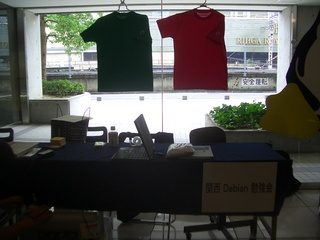
\includegraphics[width=0.5\hsize]{image200708/0720booth.jpg}
 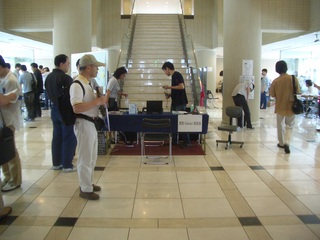
\includegraphics[width=0.5\hsize]{image200708/0721booth.jpg}
\caption{展示風景}
\label{fig:osctenjifukei}
\end{figure}

\subsection{セッション}

今回、セッションは13:00-13:45と言う45分間しかありませんでしたが、25人の
方に参加して頂きました。以下の内容について行いました。

\begin{enumerate}
 \item 関西 Debian 勉強会とは 山下 尊也
 \item Debian.org / Debian JP / 関西 Debian 勉強会の関係 矢吹 幸治
 \item Debconf 7 ミニ報告 + Debconf 日本開催について。 矢吹 幸治
\end{enumerate}

講師は、DebianJP会員であり、関西 Debian 勉強会について動いている私と矢吹さん
が行いました。

私のセッションは、関西 Debian 勉強会とはという題で、OSC Kansaiに参加して
頂いてる方にも、関西 Debian 勉強会に今後参加して頂けるように、参加し易い
勉強会をアピールしたかったので、いくつかの笑いを入れて説明しました。
第3回での「ブルースマン」さんのファイアーウォールフリーダムの画像や、なぜ、
関西 Debian 勉強会のシンボルが「ほっけ」であるのかを説明すると、会場から
は笑いが起こりました。

矢吹さんのセッションは、今まで、Debian JPと関西 Debian 勉強会との関係に
ついて述べる機会がなかったので、参加して頂いた方には、関係などが理解して
頂けました。具体的には、8月12日(日)に神戸研究学園都市で行われた第4回
関西 Debian 勉強会で、参加費について議論した際に、OSC Kansaiで聴いていた
ため、分かり易かったとおしゃって頂きました。ただ、今まで関西 Debian 勉
強会では、このような関係について述べる機会が少なかったため、今後機会を増
やす必要があると思いました。
また、Debconfについては、矢吹さんの Debconf で手に入れたお土産を景品にし
て、クイズを行いました。クイズ形式でしたが、手をあげて頂ける方が少なかっ
たのが残念でした。関西国際空港もありますので、関西で開催出来そうな
場所を教えていただけるように働きかけました。

\subsection{ブース企画}

\subsubsection{リアル掲示板}

今回、関西 Debian 勉強会では、みなさんの意見を付箋紙に書いてもらい、
Debian についての意見を書いてもらいました。

\begin{figure}[H]
\begin{center}
  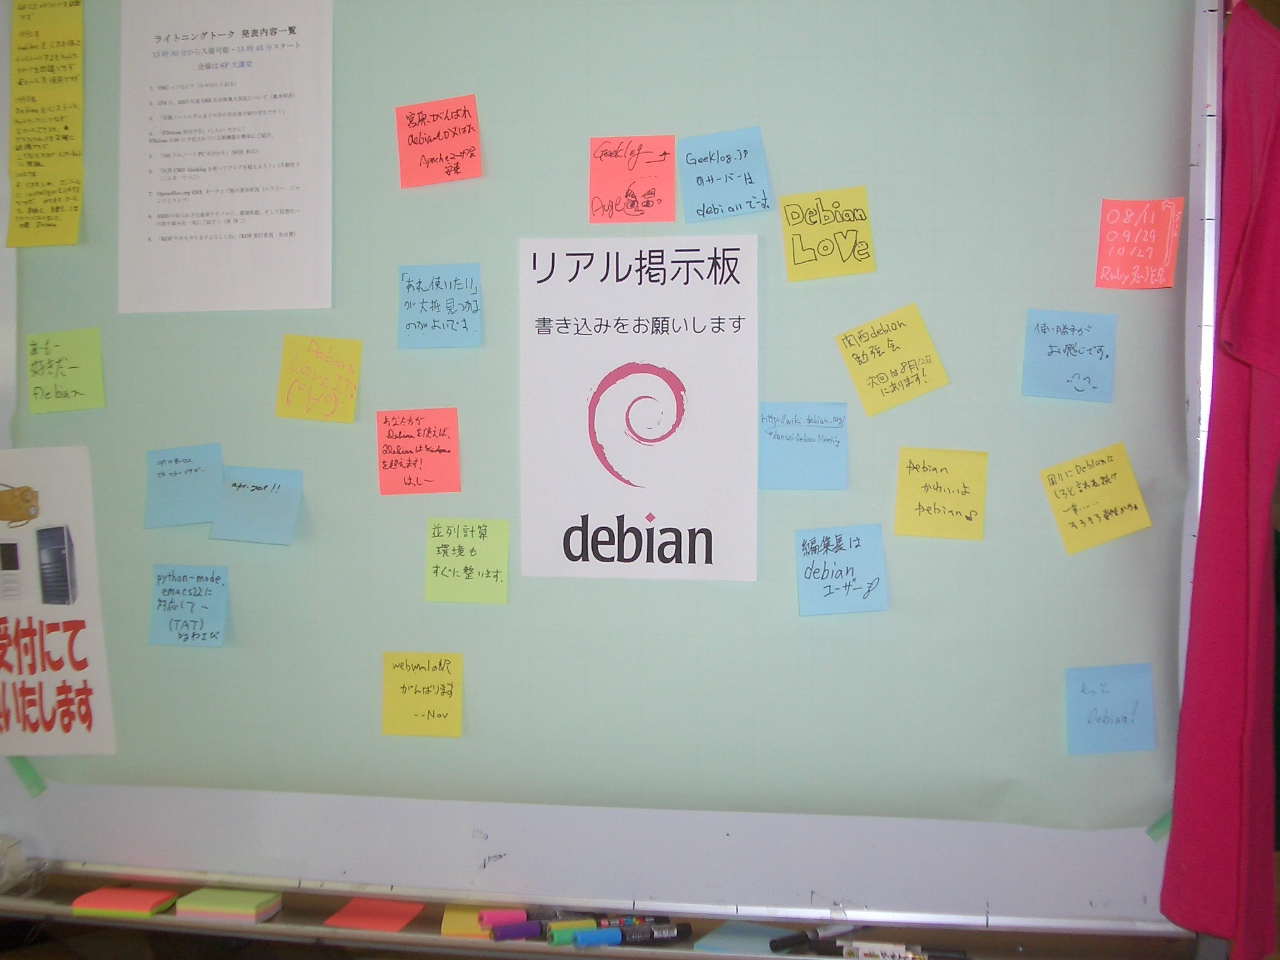
\includegraphics[width=\hsize]{image200708/real-keijiban.jpg}
\end{center}
\caption{リアル掲示板}
\label{fig:realkeiji}
\end{figure}

集まった意見は下記です。

\begin{multicols}{2}
 \begin{itemize}
 \item Debian Love IT! \verb|(・∀・)|
 \item 宮原がんばれ debian もがんばれ Apache ユーザ会 安東
 \item 「あれ使いたい」が大抵見つかるのがよいです
 \item Geeklog.JP のサーバは debian でーす。
 \item Debian Love
 \item lilo.linux.or.jp も Debian で動いています by ohura
 \item Sumibi.org も Debian で動いています! by kiyoka
 \item 編集長は Debian ユーザ!
 \item もっと Debian!
 \item Debian かわいいよ Debian ♪
 \item 使い勝手がよい感じです。
 \item 周りに Debian にしろと言われ続け一年…そろそろ覚悟かなぁ
 \item aptは使いますよ。でもマカーですが…
 \item apt-get !!
 \item python-mode emacs22 に対応してー \verb|(TAT)| by わさび
 \item webwmlの訳がんばります --Nov
 \item 並列計算環境もすぐに整います。
 \item あなた方が Debian を使えば、DebianはWindowsを越えます! はっしー
 \item あーもー好きだー Debian
 \item 1998年 Debian をインストール、ネットワークに繋ぎ、Eメールできるも、
       グラフィックカードを正確に認識できず、LYNXのみでインターネットに
       接続。
 \item 2007年 今、CDを入れ、コンソールに installguit と入力するだけで、WEBもメー
       ルも、動画も、音楽も、しほうだいになりました。万歳 Debian
 \end{itemize}
\end{multicols}

サーバでもデスクトップでも、本当にみなさん、Debian を愛してますね
\verb|:)|

個人的に気になったのは、python-modeについてですが、Emacs22から
python-modeは付属する形に変更されたみたいで、私のsid 上のEmacs22では
python-modeが動いています。

\subsubsection{配布・販売物}

以下のものを配布しました。

\begin{itemize}
 \item フライヤー
 \item DVD
\end{itemize}

\begin{center}
 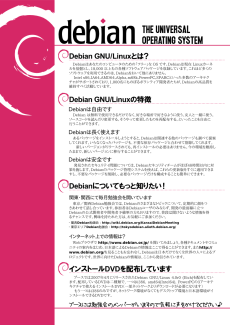
\includegraphics{image200708/flyer.png}
 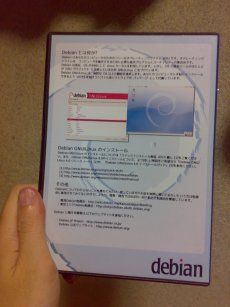
\includegraphics{image200708/dvd.jpg} 
\end{center}

関西 Debian 勉強会では、OSC Kansai で配布を行うために、矢吹さんが提案し
て頂いたフライヤーを参考に、日本人向けに作り替えるために、のがたさんがデザイン
を担当し、かがさん、倉敷さんなどが文章を考えました。

また、DVDジャケットについても、かがさんがデザインを担当し、武藤さんのイ
ンストールガイドのURLが書いてあったり、ジャケットが格好よかったので、家
に飾りますとおっしゃられた方もいらしゃいました。ただ、より多くの方に
Debian について知ってもらうために、Debian を使っていらっしゃる方
には周りの人に配布して下さいとお願いしました。

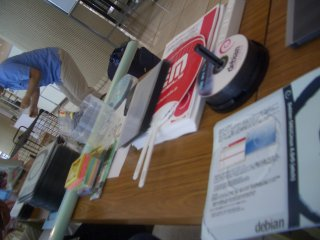
\includegraphics{image200708/booth2.jpg}
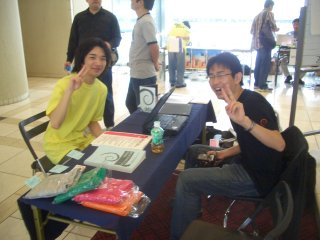
\includegraphics{image200708/booth.jpg}

以下のものを販売しました。

\begin{itemize}
 \item Tシャツ
 \item ステッカー
 \item 「あんどきゅめんてっど でびあん」2006年冬号の冊子
\end{itemize}

料金については、今年の3月に行われた OSC Spring と一緒にし、Tシャツとシー
ルは小室さん、「あんどきゅめんてっど でびあん」の冊子は岩松さんに私の家
に送って頂き、委託販売と言う形で行いました。
背景として、私が関西 Debian 勉強会に Debian Tシャツを着ていくと、やはりグッズが
欲しいなぁと言っていただいたり、紙媒体で情報が欲しいって方がいらっしゃっ
たので、実現しました。

当初、僕が予想していたものよりも多くの売り上げがあり、やはり冊子でみたい
と言う意見や、Tシャツの黒色が欲しい、Mサイズが欲しいなどの意見もありまし
たので、11月9,10日に大阪南港ATCで行われる関西オープンソースフォーラムで
もグッズの販売を行いたいと思います。

売り上げですが、Tシャツ(1枚2000円)が11枚。冊子(1部1000円)が7部。ステッ
カー(1枚300円)が12枚で、合計32,600
円(2000円*11枚+1000円*7部+300円*12枚)でした。ご協力頂いた方、本当にありがとうございました。

\dancersection{cdn.debian.or.jpの紹介}{荒木 靖宏 (yasu@debian.or.jp, ar@debian.org)}
\label{sec:cdndebianorjp}
\index{debianjp@Debian JP}
\index{cdn.debian.or.jp}
\index{Content Delivery Network}

\subsection{CDNとは}

Content Delivery Network(CDN)はウェブコンテンツ配置および配送方法として
Akamai\index{Akamai} 社によりサービスされ広く知られることになった。当初か
ら一部の人気の高いサーバへのトラフィック集中によるサーバ停止の回避、海外
のリッチコンテンツ取得の高速化、トラフィック分散によるネットワークおよび
サーバの利用平準化などの理由で広く受け入れられた。

CDNという用語自体はWWWに限ることなく、一般にコンテンツを取得するための配
送手段や方法全体を指す場合がある。たとえば、Winny\index{Winny} や
Bittorrent\index{Bittorrent}などのコンテンツを取得するために特別に設計さ
れたプロトコルを用いて、P2Pネットワークを構成するような手法も含まれる。

\subsection{DebianにおけるCDNの現状}
\subsubsection{利用法とユーザから見た動作}

\url{cdn.debian.or.jp}ではDebianでインストール時から広くdebファイルの入手に使
われるaptで使えるCDNとして設計し、運用している。そのため、Debianにおける
CDNの利用法は至極簡単である。\url{/etc/apt/source.list} に記述するAPT リポジト
リとして、

\begin{commandline}
 deb http://cdn.debian.or.jp/debian/ stable main contrib non-free
 deb-src http://cdn.debian.or.jp/debian/ stable main contrib non-free
\end{commandline}

以上のように指定するだけでユーザは今までとなんら変わることなくaptコマンド
を使用できる。サービス時の手順と構成は以下のようになる。
(\fgref{fig:usercdndebianorjp})

\begin{enumerate}
 \item  ユーザがapt-get コマンドを行うとcdn.debian.or.jpをDNSで問い合わせる
 \item  \url{cdn.debian.or.jp}を管理するDNSはサーバ候補(surrogate)選択する
 \item  選択結果をDNSのリプライとして返す
 \item  aptは\url{cdn.debian.or.jp}としてSurrogate Cを使用する
\end{enumerate}

\begin{figure}[H]
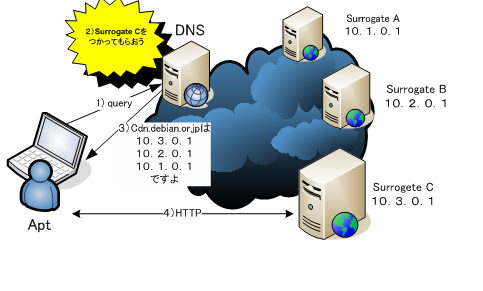
\includegraphics[width=\hsize]{image200708/surrogate.png}

 \caption{ユーザから見たcdn.debian.or.jpの動作}
 \label{fig:usercdndebianorjp}
\end{figure}

\subsubsection{cdn.debian.or.jpのシステムと動作}
CDNシステムが完全に動作しユーザから使用されるためには、システムが完全な
ファイルを提供すること、システムが安定して動作すること、そしてCDNを使っ
た場合に高速に動作していることが求められる。

\subsubsubsection{提供ファイルの完全性}

このために以下二点を満たさねばならない。
\begin{itemize}
 \item  個々のファイルがコンテンツ提供者たるdebファイル配布元と同一であること
 \item  apt-get updateの結果取得するファイル群がどのSurrogateでも入手できること
\end{itemize}
前者については、debはそのファイルのmd5値、sha1値とともに配布され、ユーザ
が使用するaptで確認後に利用されるためCDNを使用した場合でも問題にならない。

後者についてはユーザがapt-get updateを行ったときに接続するSurrogateと
apt-get dist-upgradeを行ったときに接続するSurrogateは同一であるとは限らな
いため、DNSがSurrogateとして返すサーバが保持するファイルは同一である必要
がある。\url{cdn.debian.or.jp}ではDebianプロジェクトで一般に行われている
方法と同様に、rsyncプロトコルを用い、pushミラーを行っている(図2)。その
ため、\url{cdn.debian.or.jp}のサロゲート内で最上流にあるサーバとミラーが
同一であることを2分毎にrsyncミラー終了時に作成されるスタンプファイルを確
認して、同一でないサーバはサロゲート候補から一時的に除外している。

\begin{figure}[H]
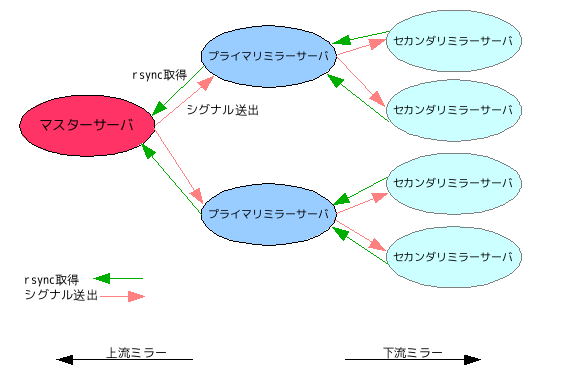
\includegraphics[width=\hsize]{image200708/pushmirror.png}
 \caption{Debianサロゲートのrsyncによるミラー}
 \label{fig:rsyncsurrogatemirror}
\end{figure}

\subsubsubsection{システムの安定動作}
先に述べたように、ユーザはCDNを使用する際にはDNSを最初に使用するため、
DNSの安定運用がカギとなる。そのため、\url{cdn.debian.or.jp}を管理するDNSサーバ
はまったく独立に動作するサーバで行っている。

また、サーバの動作を確認は、5秒以内にHTTPのレスポンスを返さないサーバは
サロゲート候補から一時的に除外している。

\subsubsubsection{高速動作}
\url{cdn.debian.or.jp}ではDNSで問い合わせされるとサロゲートリストとして複数の
IPアドレスを返す。このIPアドレスはラウンドロビンで選択しているわけではな
く、サーバキャパシティやネットワーク速度を考慮し、設定している。

\subsection{将来の展望}

ここまで説明してきた、\url{cdn.debian.or.jp}の動作には改善すべき点が多数存在す
る。改善の展望としていくつか挙げる。

\subsection{apt-getコマンドのHTTP REDIRECT}
apt-getコマンドはHTTP REDIRECTに対応していない。

HTTP REDIRECTは、いったんHTTP GETなどで接続してきたクライアントに対して、
新たにそのリソースが存在するURLを通知するものである。この仕組みをうまく
つかったCDNとして、Coral Content Distribution Network (Coral CDN)がある。
Coral CDNはサロゲート間でP2Pによるファイル配置し、そのインターフェースと
して、HTTPを使用し、しかも使用にはインターネットから取得可能なファイルで
あれば制限をかけていない。さらに、Apacheを使った一時配布サーバではHTTP
REDIRECTをつかってCoral CDNに誘導することも推奨されている。ただし、現状
で、Coral CDNを使うために、

\begin{commandline}
 deb http://cdn.debian.or.jp.nyud.net:8090/debian/ stable main contrib non-free
\end{commandline}
を指定することも可能だが、少なくとも日本においてはCoral CDNを担うサロゲー
トが存在しないこともあって非常に低速である。ただし韓国や中国では広くつか
われており、将来の拡張に使用したい。

\subsubsection{IPアドレスの位置情報を使用したサーバ選択}

globalにCDNを展開する場合には地理的に近いサーバ群からある程度絞込むのが
有効である。現在、GeoIPなど無料でIPと地理情報のマッピング提供者が現れて
おり、この活用は\url{cdn.debian.or.jp}の次の拡張として最有力だと考えている。

\subsubsection{aptのP2P対応}

現在、\url{http://wiki.debian.org/DebTorrent} や
\url{http://www.cs.sfu.ca/~camerond/personal/GoogleSoCDebian.html}でaptの
Bittorrent対応が進められており、有力な候補である。ただし、Bittorrentプロ
トコルをクライアントで直接使うものであり、ネットワーク利用ポリシーとの競
合やinstall時に利用可能なのかなど今後検証すべき問題も多い。


\subsection{おわりに}

いつでも必要なソフトウェアやコンテンツを安価に入手する手段としてCDNはこ
れからも様々な発展を続けると考える。Debianはdebの安定入手手段の有無がシ
ステムの信頼性を左右するシステムであり、CDNの広範な活用が今後ますます求
められるようになると考える。


\dancersection{Debian GNU/kFreeBSD のインストール}{上川 純一}
\label{sec:debiankfreebsd}
\index{FreeBSD}
\index{Debian GNU/kFreeBSD}

\subsection{はじめに}

最近めっきり話題の Debian GNU/kFreeBSD を qemu でインストールしてみました。

\subsection{CDイメージの取得}

Debian GNU/kFreeBSDのページ
\url{http://www.debian.org/ports/kfreebsd-gnu/}からリンクをたどり、今回は
\url{http://glibc-bsd.alioth.debian.org/install-cd/kfreebsd-i386/20070313/}
から debian-20070313-kfreebsd-i386-install.iso を取得しました。

\url{http://glibc-bsd.alioth.debian.org/doc/} に文書があります。

\subsection{qemu の準備}

まず、ディスクイメージを作成します。

\begin{commandline}
qemu-img create -f qcow f.cow 4G
\end{commandline}

\subsection{インストーラの起動}

qemu で ISO イメージから起動します。具体的なコマンドラインはこのようにな
ります。(筆者のシステムは amd64 アーキテクチャのため、 kqemu を活用する
ために、qemu-system-x86\_64 を利用しています。i386であれば、 qemu コマンド
をかわりに利用します。)

\begin{commandline}
qemu-system-x86_64 -hda f.cow \
 -cdrom debian-20070313-kfreebsd-i386-install.iso \
 -m 256 -boot d 
\end{commandline}



Expressを選択、適当にパーティションを切ってみて、FreeBSDのブートローダを
利用してみました。マニュアルにしたがって適当に答えていきます。
インストール対象は Minimal を選択して、インストールを続行します。

\begin{figure}[H]
 \begin{multicols}{2}
 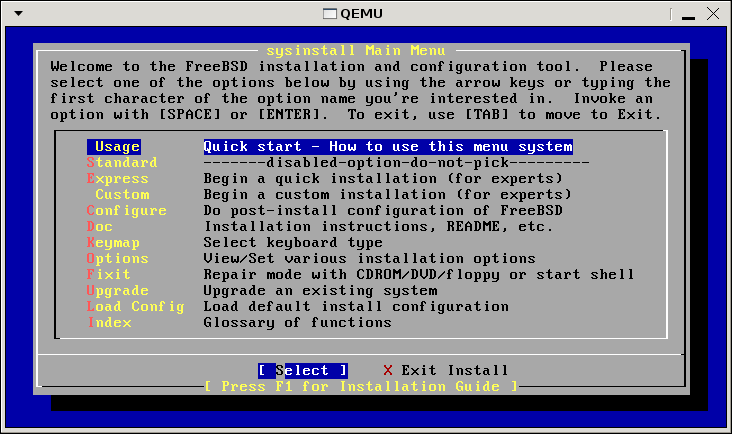
\includegraphics[width=\hsize]{image200708/kfreebsd-install-0.png}
 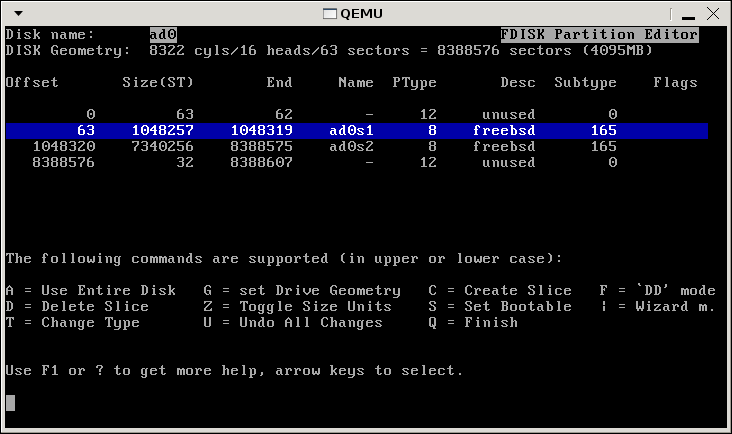
\includegraphics[width=\hsize]{image200708/kfreebsd-install-1.png}
 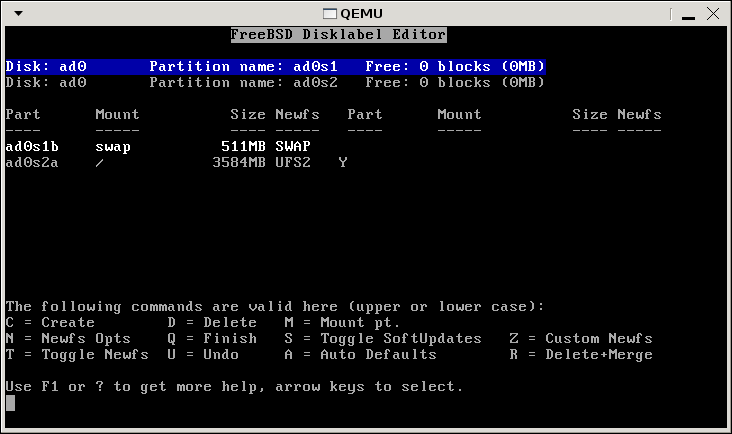
\includegraphics[width=\hsize]{image200708/kfreebsd-install-2.png}
 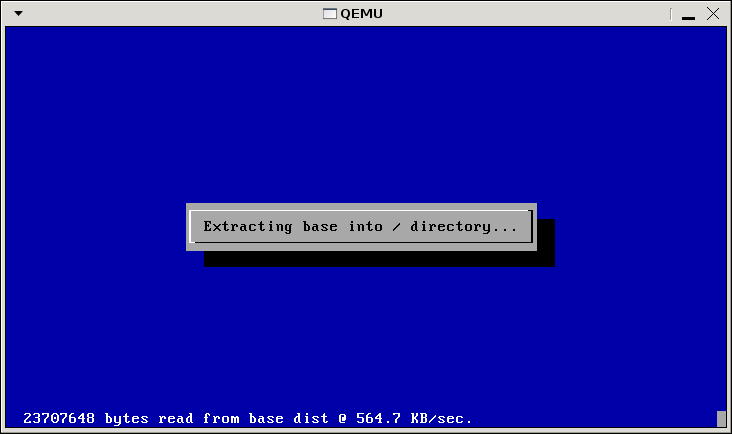
\includegraphics[width=\hsize]{image200708/kfreebsd-install-3.png}
 \end{multicols}
\caption{Debian GNU/kFreeBSD インストール画面}
\label{fig:kfreebsdinst}
\end{figure}

しばらく待つと alt-f3 で画面を切り替えろと表示されます。
debconf の質問に答つつインストールがつづきます。

\begin{figure}[H]
 \begin{center}
  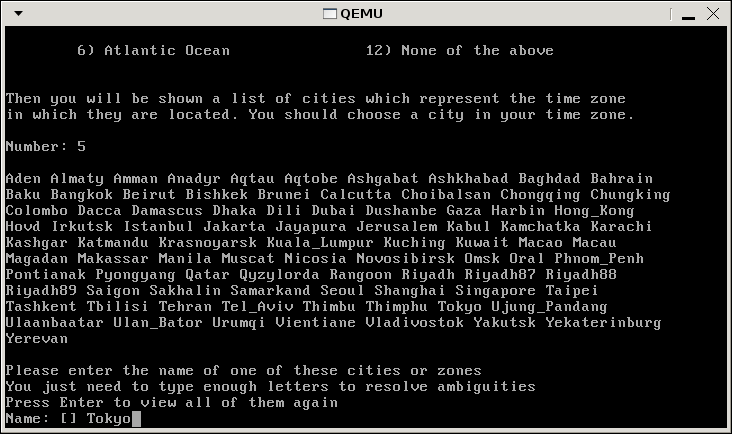
\includegraphics[width=0.5\hsize]{image200708/kfreebsd-install-4.png}
 \end{center}
 \caption{初期パッケージインストール・設定中}
 \label{fig:kfreebsdinst2}
\end{figure}

最後にリブートをするように指示されるので、そこで
qemu を一旦終了します。

ここで、 qemu を HDD イメージから起動するようにして実行します。

\begin{commandline}
 qemu-system-x86_64 -hda f.cow -m 256 
\end{commandline}

起動すると、なぜだか root filesystem が read-only だからといろいろと失敗
します。
fsck が必要な場合の起動に不都合があるようです。
一旦 root でログインし、reboot コマンドでリブートしてみると root
filesystem を正常にマウントすることが出来るようです。

また、 /etc/network/interfaces がまったく設定されていない状態なので、ネットワー
クが使えない状態で起動してきますが dhclient を実行すればIPを取得して稼働
することも可能です。

\begin{commandline}
 dhclient ed0
\end{commandline}

\subsection{動いた!}

これで無事に Debian GNU/kFreeBSD の稼働が確認できました。
まだまだ完成度が至らない点が多いので、デバッグしほうだいです。

 \begin{figure}[H]
  \begin{center}
   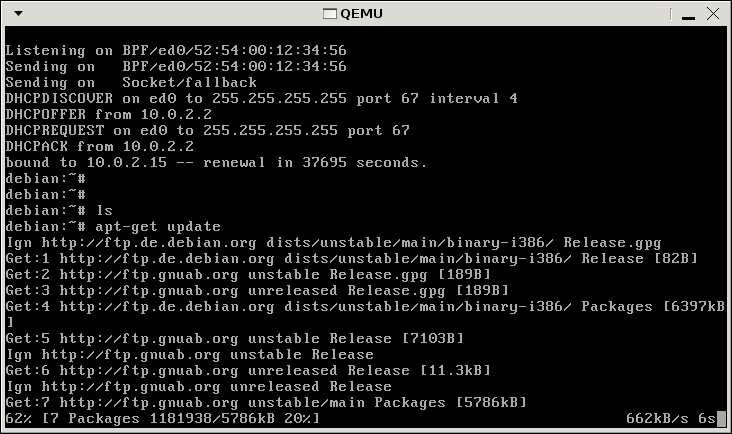
\includegraphics[width=0.5\hsize]{image200708/kfreebsd-install-5.png}
  \end{center}
  \caption{Debian GNU/kFreeBSD で apt-get してみました}
  \label{fig:kfreebsdaptget}
 \end{figure}

\dancersection{今後の予定}{上川 純一}

\subsection{次回}
次回は9月15日に東京エリアDebian勉強会があります。

\subsection{OSC Tokyo/Fall}

10月5日・6日に開催されます。Debian JPも「東京エリアDebian勉強会」として
参加します。

%\printindex

\cleartooddpage

\begin{minipage}[b]{0.2\hsize}
 \colorbox{dancerlightblue}{\rotatebox{90}{\fontsize{80}{80} {\gt デビアン勉強会} }}
\end{minipage}
\begin{minipage}[b]{0.8\hsize}

\vspace*{15cm}
{\color{dancerlightblue}\rule{\hsize}{1mm}}
\vspace{2mm}

\includegraphics[width=2cm]{image200502/openlogo-nd.eps}
\noindent \Large \bf Debian 勉強会資料\\ \\
\noindent \normalfont \debmtgyear{}年\debmtgmonth{}月\debmtgdate{}日 \hspace{5mm}  初版第1刷発行\\
\noindent \normalfont 東京エリア Debian 勉強会 (編集・印刷・発行)\\
{\color{dancerdarkblue}\rule{\hsize}{1mm}}
\end{minipage}

\end{document}
